%% start of file `template.tex'.
%% Copyright 2006-2015 Xavier Danaux (xdanaux@gmail.com).
%
% This work may be distributed and/or modified under the
% conditions of the LaTeX Project Public License version 1.3c,
% available at http://www.latex-project.org/lppl/.


\documentclass[11pt,a4paper,sans]{moderncv}        % possible options include font size ('10pt', '11pt' and '12pt'), paper size ('a4paper', 'letterpaper', 'a5paper', 'legalpaper', 'executivepaper' and 'landscape') and font family ('sans' and 'roman')
\usepackage{ragged2e}
\usepackage{lastpage}
\usepackage[german]{babel} 
\usepackage{fancyhdr}
%\renewcommand{\refname}{Articles}
\addto\captionsgerman{\renewcommand\refname{Publications}}

\fancyfoot[C]{ \thepage\ / 6}
\usepackage{pdfpages}
% moderncv themes
\moderncvstyle{classic}
\usepackage{xpatch}
\xpatchcmd{\makeletterclosing}{[3em]}{[2em]}{}{}%abstand nach closing                           % style options are 'casual' (default), 'classic', 'banking', 'oldstyle' and 'fancy'
\moderncvcolor{blue}                               % color options 'black', 'blue' (default), 'burgundy', 'green', 'grey', 'orange', 'purple' and 'red'
%\renewcommand{\familydefault}{\sfdefault}         % to set the default font; use '\sfdefault' for the default sans serif font, '\rmdefault' for the default roman one, or any tex font name
%\nopagenumbers{}                                  % uncomment to suppress automatic page numbering for CVs longer than one page

% character encoding
%\usepackage[utf8]{inputenc}                       % if you are not using xelatex ou lualatex, replace by the encoding you are using
%\usepackage{CJKutf8}                              % if you need to use CJK to typeset your resume in Chinese, Japanese or Korean
\renewcommand*{\namefont}{\fontsize{20}{40}\mdseries\upshape}

% adjust the page margins
\usepackage[scale=0.75]{geometry}
%\setlength{\hintscolumnwidth}{3cm}                % if you want to change the width of the column with the dates
%\setlength{\makecvtitlenamewidth}{10cm}           % for the 'classic' style, if you want to force the width allocated to your name and avoid line breaks. be careful though, the length is normally calculated to avoid any overlap with your personal info; use this at your own typographical risks...



% personal data
\name{Fabian E.}{Gruber}
%\title{Resumé title}                               % optional, remove / comment the line if not wanted
\address{Anna-Stainer-Knittel-Weg 3/5/4}{6020 Innsbruck, Austria}% optional, remove / comment the line if not wanted; the "postcode city" and "country" arguments can be omitted or provided empty
\phone[mobile]{+43~650~2587521}                   % optional, remove / comment the line if not wanted; the optional "type" of the phone can be "mobile" (default), "fixed" or "fax"
%\phone[fixed]{+2~(345)~678~901}
%\phone[fax]{+3~(456)~789~012}
\email{Fabian.Gruber@uibk.ac.at}                               % optional, remove / comment the line if not wanted
%\homepage{www.johndoe.com}                         % optional, remove / comment the line if not wanted
%\social[linkedin]{john.doe}                        % optional, remove / comment the line if not wanted
%\social[twitter]{jdoe}                             % optional, remove / comment the line if not wanted
%\social[github]{jdoe}                              % optional, remove / comment the line if not wanted
%\extrainfo{additional information}                 % optional, remove / comment the line if not wanted
\photo[64pt][0.2pt]{fabian_bewerbungsfoto}                       % optional, remove / comment the line if not wanted; '64pt' is the height the picture must be resized to, 0.4pt is the thickness of the frame around it (put it to 0pt for no frame) and 'picture' is the name of the picture file
%\quote{}                                 % optional, remove / comment the line if not wanted

% bibliography adjustements (only useful if you make citations in your resume, or print a list of publications using BibTeX)
%   to show numerical labels in the bibliography (default is to show no labels)
\makeatletter\renewcommand*{\bibliographyitemlabel}{\@biblabel{\arabic{enumiv}}}\makeatother
%   to redefine the bibliography heading string ("Publications")
%\renewcommand{\refname}{Articles}
%\addto\captionsenglish{\renewcommand\refname{Publications}}

% bibliography with mutiple entries
%\usepackage{multibib}
%\newcites{book,misc}{{Books},{Others}}
%----------------------------------------------------------------------------------
%            content
%----------------------------------------------------------------------------------
\begin{document}
%\begin{CJK*}{UTF8}{gbsn}                          % to typeset your resume in Chinese using CJK

%-----       letter       ---------------------------------------------------------
% recipient data
\recipient{Dr. Peter Arndorfer}{Austrian Centre for Digital Humanities \\Austrian Academy of Sciences\\Sonnenfelsgasse 19/8\\A-1010 Vienna}
\date{February 13, 2018}
\opening{\textbf{Subject: Application as Data Curator} \\[0.5cm]     Dear Dr. Arndorfer,}
\closing{Best regards,}
\enclosure[Attached]{Resume, List of publications, References and Diploma Certificate}          % use an optional argument to use a string other than "Enclosure", or redefine \enclname
\makelettertitle
\justify
After several years as a research assistant at the Institute of Geography of the University of Innsbruck, I am currently writing my PhD Thesis and relocating to Vienna. The advertised position as data curator  appeals to me in that it presents the possibility to continue working in my main field of expertise, geographic information systems and geodata management. Additionally, due to the part time nature of the position, it would allow me to finish my thesis with the title \emph{Terrain analysis to support field soil survey}.

Geographic information systems and geodata management have played a major part in my work as a research assistant, both at the University of Natural Resources and Life Sciences and the University of Innsbruck. After beginning with ArcGIS, I have now specialised on the use of Open Source systems such as GRASS, SAGA and QGIS, the latter mainly for visualising geospatial data, especially in vector format. Applying these Open Source GIS has also given me profound insight into the functioning of GIS. While scripting with Python allows me to be more efficient in computing with, and combining, these different GIS, the use of R, a free software environment for statistical computing and graphics, has improved my  abilities to analyse geospatial data. Researching available spatial data in South Tyrol has shown me the great possibilities, but also limitations, of the use of historical maps such as the Franziscean Cadastre in research projects.  

In addition to my experience with GIS and the management of spatial data from different sources, I am also used to, and enjoy, working in teams made up of experts from different fields of expertise. I have enclosed a resume and references, and would enjoy discussing this position at your
convenience. Should you require any additional material or information, I am happy to supply it.

Thank you for your consideration.



\makeletterclosing
\clearpage
%-----       resume       ---------------------------------------------------------
\makecvtitle


\section{Experience}
\subsection{Vocational}
\cventry{2013--2018}{Research Assistant}{Institute of Geography, University of Innsbruck}{Innsbruck}{}{Research projects: 
\begin{itemize}%
\item Shallow erosion dynamics in mountain grasslands of South Tyrol: Monitoring, process analysis and mitigation measures (EroDyn)
  \begin{itemize}%
  \item Geodata management: aquisition and storage of available geospatial data
  \item Accuracy assessment for geographical object-based modelling of land cover with Python and Open Source GIS
  \item Regional-scale landslide susceptibility mapping
  \end{itemize}
\item Terrain Classification
of ALS Data to support Digital Soil Mapping
  \begin{itemize}%
  \item Landform delineation with statistical learning approaches and automated landform classifications
  \item Field Soil Survey
  \item Collaboration on the development of the Java App \emph{SEPP (Soil Evaluation in Planning Procedures)}
  \end{itemize}
\end{itemize}
}
\cventry{2011--2013}{Research Assistant}{Institute of Applied Geology,  BOKU}{Vienna}{}{Research projects: 
\begin{itemize}%
\item Hazard assessment for an expected dam break flood in the Hunza Valley, Pakistan: A combination of GIS, Remote Sensing, and computer simulation techniques
\begin{itemize}%
  \item Dam breach modeling with BREACH
  \item Flood modeling with FLO-2D
  \end{itemize}
\item Poverty Alleviation through Mitigation of Integrated High-Mountain Risk (PAMIR)
\begin{itemize}%
  \item Mapping geomorphological hazards, glaciers, and vulnerable infrastructure with remotely sensed data 
  \end{itemize}
  \end{itemize}}
\cventry{2009--2010}{Project Assistant}{Institute of Applied Geology,  BOKU}{Vienna}{}{Research project: 
\begin{itemize}%
\item Remote Geohazards Assessment in Tajikistan (TajHaz)
\begin{itemize}%
  \item Mapping geomorphological hazards and glacial lakes with remotely sensed data 
  \item Field survey in Tajikistan
  \end{itemize}
  \end{itemize} }

\subsection{Miscellaneous}
\cventry{2016--2017}{Educational Leave (Bildungskarenz)}{}{}{}{devoted to work on PhD thesis with the working title 'Digital terrain analysis to support field soil survey'}
\cventry{2016--2017}{Lecturer}{Institute of Geography, University of Innsbruck}{Innsbruck}{}{Exercises in Statistics ({\"U}bungen zur Statistik): Introduction to statistics with R for Bachelor's students}
\cventry{2010--2011}{Student tutor}{University of
Natural Resources and Life Sciences (BOKU) }{Vienna}{}{Tutoring for students using ArcGIS}

\section{Master thesis}
\cvitem{title}{\emph{The 2010 Attabad Landslide Dam Lake:
modeling and prediction of Lake Outburst
Floods}}
\cvitem{supervisors}{Jean F. Schneider and Martin Mergili}

\section{Education}
\cvitem{2002--2011}{Diploma Study of Environmental Engineering
and Water Management at the University of
Natural Resources and Life Sciences (BOKU), Vienna
}
\cvitem{1993--2001}{Linz International School Auhof, Linz:
Austrian Matura (school leaving certificate,
university entry qualification) and International
Baccalaureate (IB)}
\cvitem{1991--1993}{Elementary School Linz-Pichling}
\cvitem{1989--1991}{Lincoln Elementary School Pittsburgh, PA, USA}



\section{Languages}
\cvitem{German}{Native Language}{ }
\cvitem{English}{Fluent}{ }
\cvitem{Spanish}{Conversant}{ }
\cvitem{French}{Conversant}{ }

\section{Computer skills}
\cvdoubleitem{Operating systems}{Windows, Linux (Ubuntu)} {Scripting}{R, Python, Bash}
\cvdoubleitem{Geographic information systems}{GRASS, QGIS, SAGA, ARCGIS} {Word processing} {MS Word, Libreoffice ,  \LaTeX{} with Texmaker}
\cvdoubleitem{Image processing}{GIMP, Inkscape}{Misc. software}{RStudio, MS Office, FLO-2D, ENVI-Sarscape}
\section{Interests}
\cvitem{Horticulture}{Participating in a communal gardening project}
\cvitem{Traveling}{Extensive traveling in Central and South America, Central Asia, Southeast Asia and Madagascar}

% Publications from a BibTeX file without multibib
%  for numerical labels: \renewcommand{\bibliographyitemlabel}{\@biblabel{\arabic{enumiv}}}% CONSIDER MERGING WITH PREAMBLE PART
%  to redefine the heading string ("Publications"): \renewcommand{\refname}{Articles}
\nocite{*}
\bibliographystyle{plain}
\clearpage
\bibliography{publications3}
%\clearpage  
 
\subsection{Peer-reviewed journal articles and book chapters}
\cvitem{[1]}{Gruber, F.E., Baruck, J., Geitner, C. (2017):  Algorithms vs. surveyors: a comparison of automated landform delineations and surveyed topographic positions from soil mapping in an Alpine environment. Geoderma 308, 9-25.}
\cvitem{[2]}{Geitner, C., Baruck, J., Freppaz, M., Godone, D., Grashey-Jansen, S., Gruber, F.E., Heinrich, K., Papritz, A., Simon, A., Stanchi, S., Traidl, R., von Albertini, N., Vrscaj, B. (2017). Soil and land use in the Alps -- Challenges and examples of soil survey and soil data use to support sustainable development. In: Pereira, P., Brevik, E.C., Munoz-Rojas, M., Miller, B. (Eds.), Soil mapping and process modelling for sustainable land use management. Elsevier, Amsterdam. 221-292}
\cvitem{[3]}{Baruck, J., Nestroy, O., Sartori, G., Baize, D., Traidl, R., Vrisaj, B., Br{\"a}m, E., Gruber, F.E., Heinrich, K., Geitner, C. (2016): Soil classification
and mapping in the Alps: The current state and future challenges.
Geoderma 264, Part B, 312--331.}
\cvitem{[4]}{Zieher, T., Gruber, F.E.; Rutzinger, M.; Mei{\ss}l, G.; Geitner, C.; Perzl, F. (2016): Data
requirements for the assessment of shallow landslide susceptibility using logistic regression. In: Proceedings of the 12th International Symposium on Landslides - Landslides and Engineered Slopes. Experience, Theory and Practice. Napoli, Italy. CRC Press, S. 2139-2146.}
\cvitem{[5]} {Gruber, F.E., Mergili, M. (2013): Regional-scale analysis of high-mountain multi-hazard and risk indicators in the Pamir (Tajikistan) with GRASS GIS. Natural Hazards and Earth System Sciences 13: 2779-2796.}
\cvitem{[6]} {Schneider, J.F., Gruber, F.E., Mergili, M. (2013): Impact of large landslides, mitigation measures. In: Genevois, R., Prestininzi, A. (eds.): International Conference on Vajont - 1963-2013 - Thoughts and analyses after 50 years since the catastrophic landslide. Proceedings of the International Conference Vajont 1963-2013, Padua, Italy, October 8-10, 2013. Italian Journal of Engineering Geology and Environment - Book: 73-84.}
\cvitem{[7]} {Schneider, J.F., Gruber, F.E., Mergili, M. (2013): Recent Cases and Geomorphic Evidence of Landslide-Dammed Lakes and Related Hazards in the Mountains of Central Asia. In: Margottini, C., Canuti, P., Sassa, K. (eds.): Landslide Science and Practice: Volume 6: Risk Assessment, Management and Mitigation (Proceedings of the 2nd World Landslide Forum, FAO Headquarters Rome, Italy, October 3-9, 2011): 57-64. Springer, Heidelberg, Berlin, New York}
\subsection{Selected conference abstracts and presentations}
\cvitem{[8]}{Gruber, F.E., Baruck, J. und C. Geitner (2016): Joint analysis of parent material and topography to support soil survey -- a case study from South Tyrol.  Jahrestagung
der {\"O}sterreichischen Forschungsgruppe f{\"u}r Geomorphologie und Umweltwandel und der Schweizerischen Gesellschaft f{\"u}r Geomorphologie 2016, Innsbruck (23.09.2016).}
\cvitem{[9]}{Gruber F.E., Baruck, J., Simon, A. und C. Geitner (2015): Reliefklassifizierung f{\"u}r die
Erstellung von Bodenkarten anhand von geomorphons (GRASS GIS).--  Posterausstellung im Rahmen der Jahrestagung der Deutschen Bodenkundlichen Gesellschaft, M{\"u}nchen 2015, AG Digital Soil Mapping (09.09.2015). }
\cvitem{[10]}{Gruber, F.E., Zieher, T., Rutzinger, M. und C. Geitner (2015): Geomorphons and structure metrics for the characterization of geomorphological landscape regions in Austria. EGU General Assembly 2015 (EGU 2015), Wien
(16.04.2015).  }
\cvitem{[11]}{Gruber, F.E., Baruck, J., Rutzinger, M. and C. Geitner (2014): Landform segmentation for
digital soil mapping. -- EGU General Assembly 2014 (28.04.-02.05.2014, Vienna (Austria)), Geophysical Research Abstracts Vol. 16, EGU2014-5644.  }
                   % 'publications' is the name of a BibTeX file

% Publications from a BibTeX file using the multibib package
%\section{Publications}
%\nocitebook{book1,book2}
%\bibliographystylebook{plain}
%\bibliographybook{publications}                   % 'publications' is the name of a BibTeX file
%\nocitemisc{misc1,misc2,misc3}
%\bibliographystylemisc{plain}
%\bibliographymisc{publications}                   % 'publications' is the name of a BibTeX file
%\clearpage
\vspace{20mm}
\section{References}


\begin{tabular}{lr}
% Referee 1
\begin{minipage}[t]{3.5in}
Privat.-Doz.Dr. \ Martin Mergili\\
Institute of Applied Geology (IAG)\\
University of Natural Ressources and Life Sciences\\
Peter-Jordan-Stra{\ss}e 82\\
1190 Vienna, Austria\\
\phonesymbol +43 1 47654 87219\\
\emailsymbol \href{mailto:martin.mergili@boku.ac.at}{martin.mergili\textrm{@}boku.ac.at}
\end{minipage}
&
% Referee 2
\begin{minipage}[t]{3.0in}
Assoz.Univ-Prof Dr.\ Clemens Geitner\\
Institute of Geography\\
University of Innsbruck\\
Innrain 52f\\
6020 Innsbruck, Austria\\
\phonesymbol +43 512 507 5437\\
\emailsymbol \href{mailto:clemens.geitner@uibk.ac.at}{clemens.geitner\textrm{@}uibk.ac.at}
\end{minipage}
\\
\\ % Additional newline for spacing.
% Referee 3
\begin{minipage}[t]{4in}
Privat.-Doz.Dr.\ Martin Rutzinger\\
Institute of Interdisciplinary Mountain Research\\
Austrian Academy of Sciences\\
Technikerstra{\ss}e 21a \\
6020 Innsbruck, Austria\\
\phonesymbol +43 512 507 49480\\
\emailsymbol \href{mailto:martin.rutzinger@oeaw.ac.at}{martin.rutzinger\textrm{@}oeaw.ac.at}
\end{minipage}
\end{tabular}

\clearpage
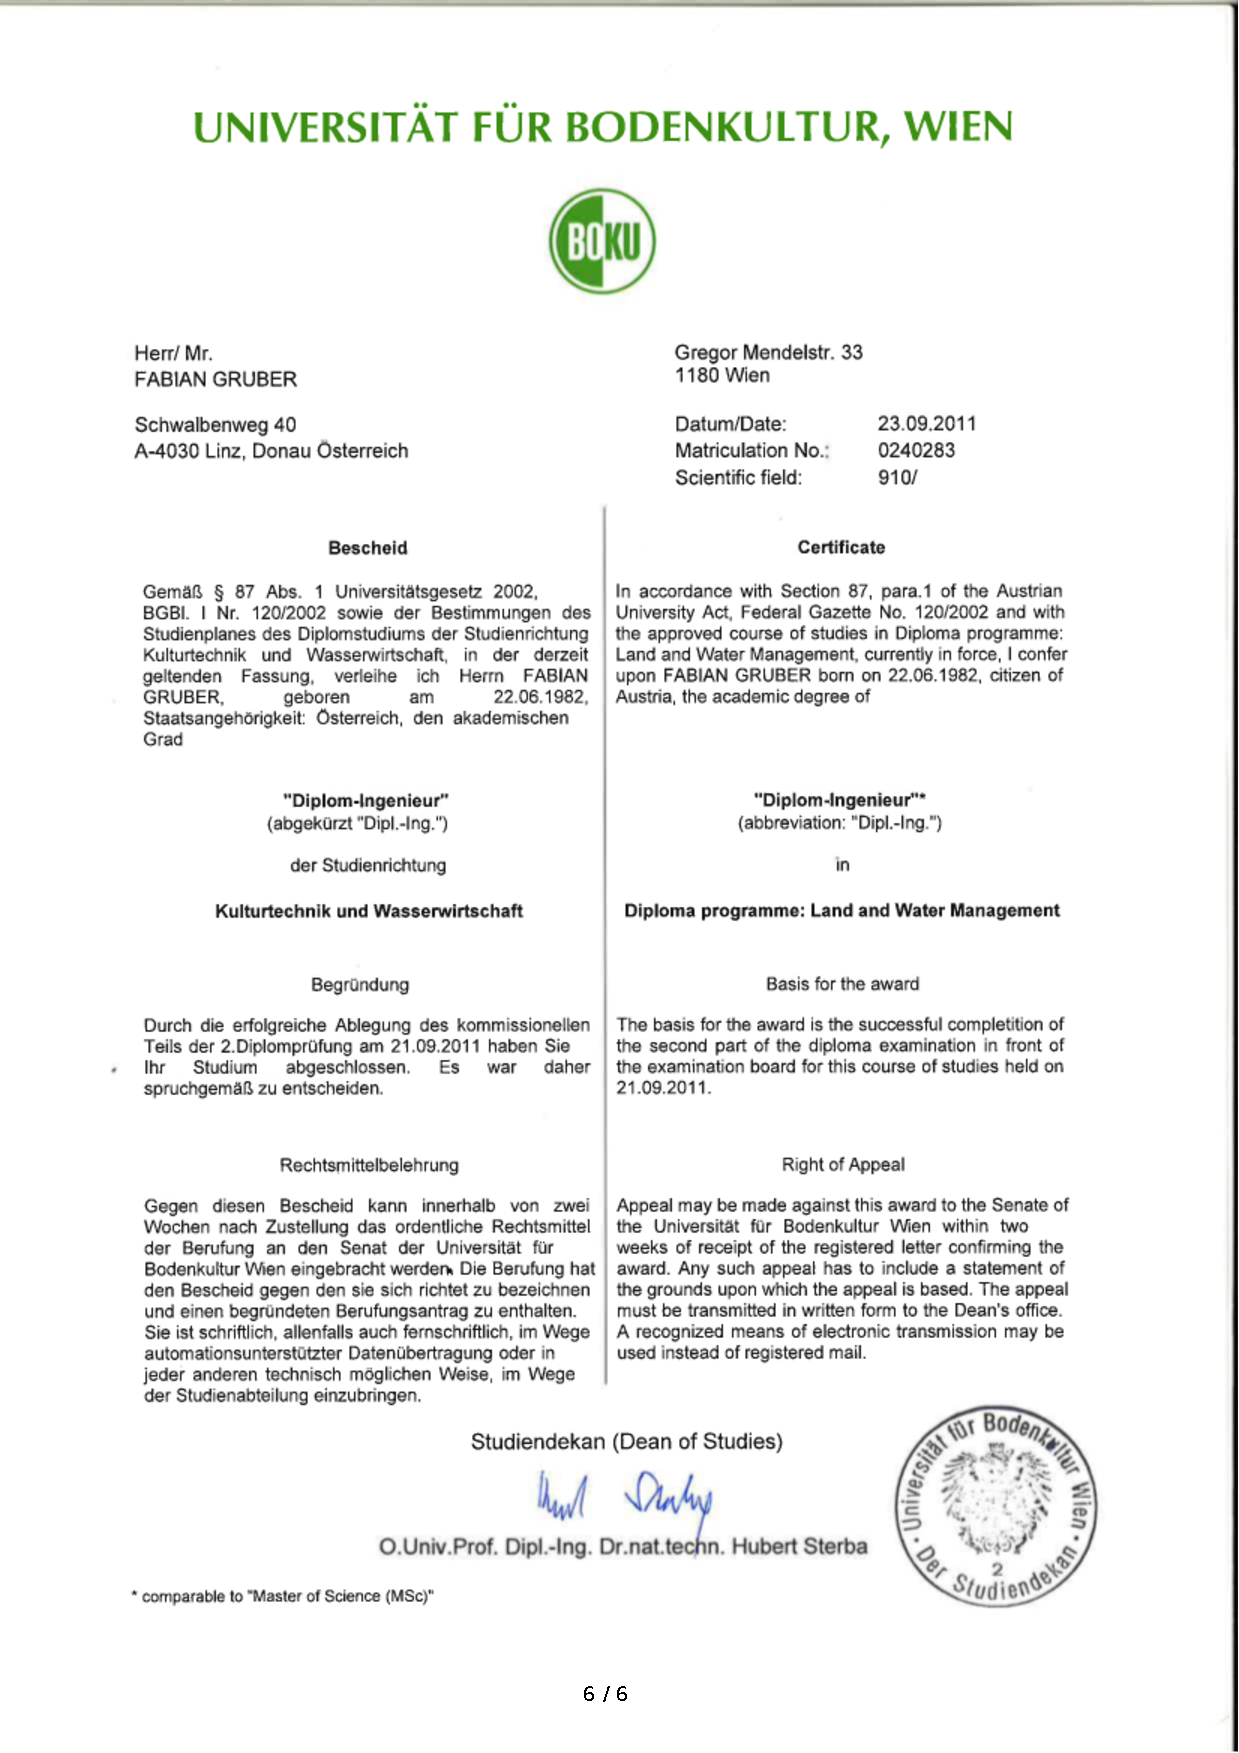
\includepdf{DP_6vonv.pdf}
%\clearpage\end{CJK*}                              % if you are typesetting your resume in Chinese using CJK; the \clearpage is required for fancyhdr to work correctly with CJK, though it kills the page numbering by making \lastpage undefined
\end{document}


%% end of file `template.tex'.
